\documentclass[journal]{IEEEtran}
\usepackage[a5paper, margin=10mm]{geometry}
%\usepackage{lmodern} % Ensure lmodern is loaded for pdflatex
\usepackage{tfrupee} % Include tfrupee package


\setlength{\headheight}{1cm} % Set the height of the header box
\setlength{\headsep}{0mm}     % Set the distance between the header box and the top of the text


%\usepackage[a5paper, top=10mm, bottom=10mm, left=10mm, right=10mm]{geometry}

%
\usepackage{gvv-book}
\usepackage{gvv}
%\setlength{\intextsep}{10pt} % Space between text and floats

\makeindex

\begin{document}
\bibliographystyle{IEEEtran}
\onecolumn


\title{
	%\begin{flushleft}
	\begin{center}
	%MATRICES \\ In Geometry
	POMPS
	\\
\rule{0.4\columnwidth}{0.4pt}
%\end{flushleft}
\end{center}
}
\author{
\vspace{11cm}
	%\begin{flushleft}
	\begin{center}
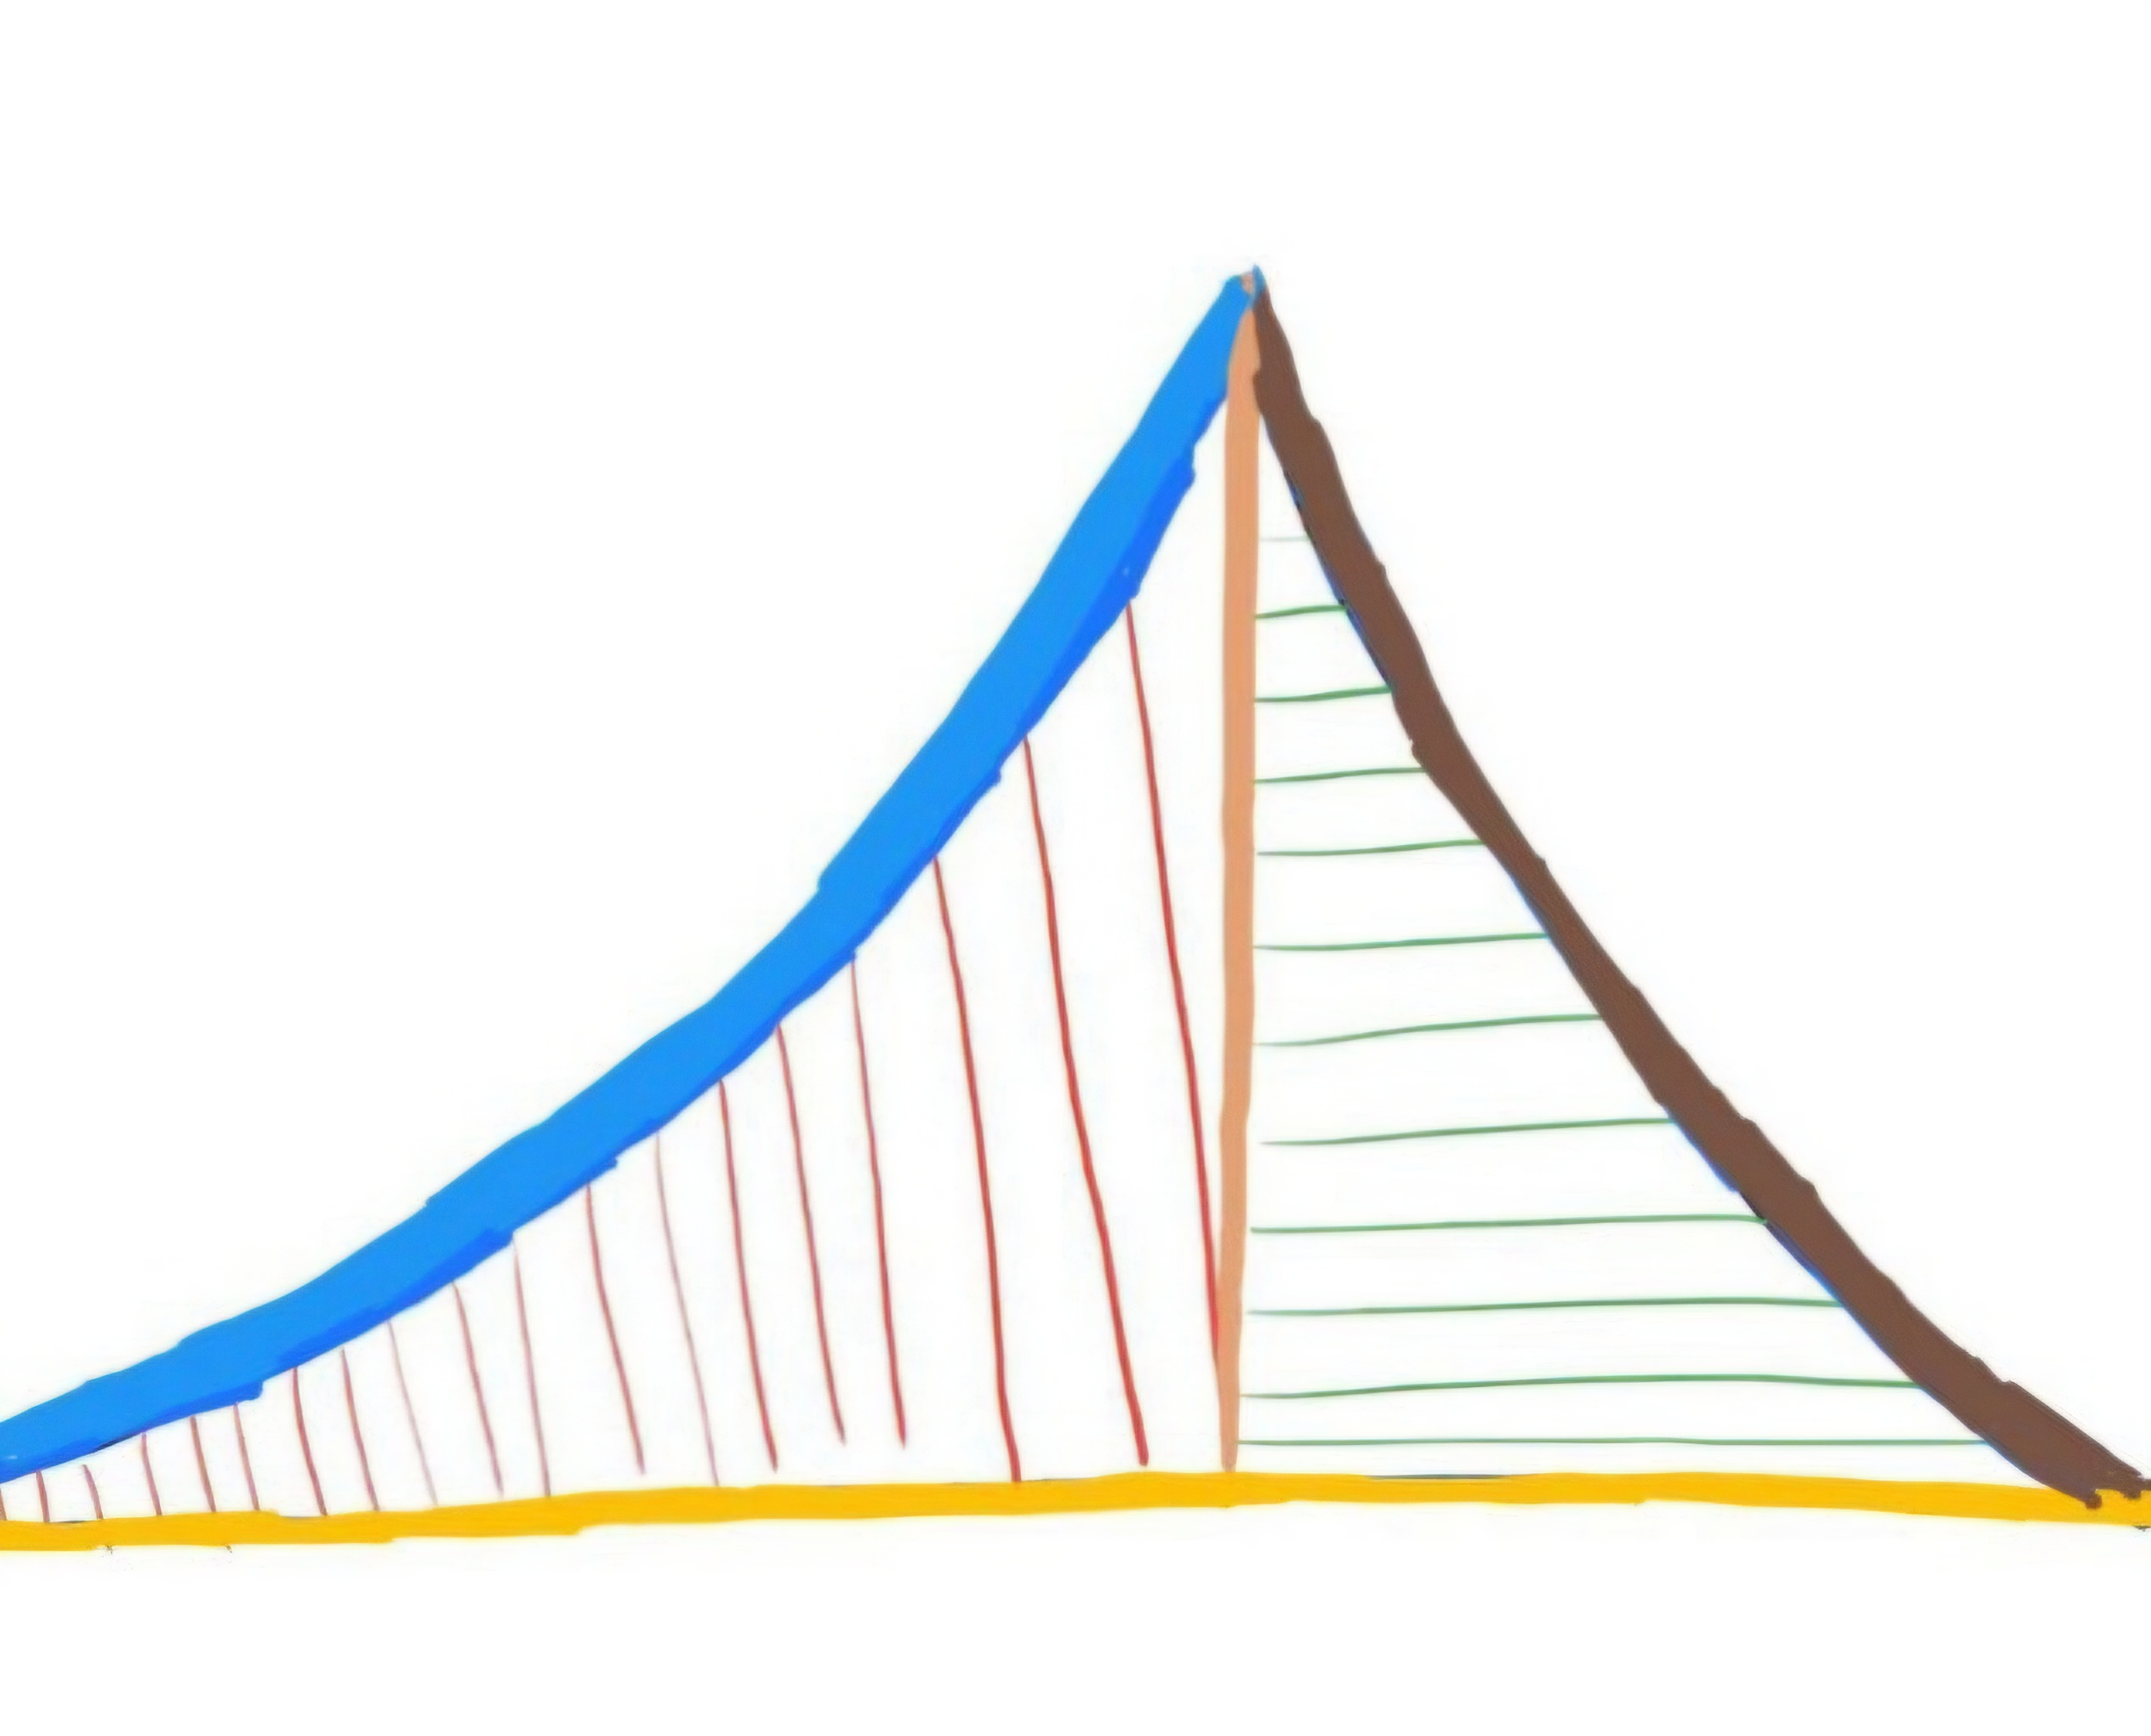
\includegraphics[width=0.2\columnwidth]{figs/logo.jpg}
\\
		{	\huge G. V. V. Sharma}
	\end{center}
	%\end{flushleft}
%\IEEEpubid{\makebox[\columnwidth]{978-1-7281-5966-1/20/\$31.00 ©2020 IEEE \hfill} \hspace{\columnsep}\makebox[\columnwidth]{ }}
}
\maketitle

\newpage
\section*{About this Book}

This book introduces matrices through high school coordinate geometry. This approach makes it easier for beginners to learn Python for scientific computing. All problems in the book are from NCERT mathematics textbooks from Class 9-12.  Exercises are from CBSE board exam papers.   

The content is sufficient for industry jobs and covers nearly all matrix prerequisites for machine learning.
There is no copyright, so readers are free to print and share.  

%This book is dedicated to my high school teachers, Dr. G.N. Chandwani and Dr. Anand K. Tripathi.
%\begin{flushright}
%\today
%\end{flushright}
%Github: https://github.com/gadepall/matgeo
%		\\
License: https://creativecommons.org/licenses/by-sa/3.0/
\\
and
\\
https://www.gnu.org/licenses/fdl-1.3.en.html
\\
First manual appeared in January 2018
\\
First edition published on July 10, 2024
\\
In this edition, some incorrect solutions were removed.  All figures redrawn. More problems added.

\newpage


\tableofcontents

\newpage
%\twocolumn
\onecolumn


%\renewcommand{\theequation}{\theenumi}
\numberwithin{equation}{enumi}
\numberwithin{figure}{enumi}
%\renewcommand{\thefigure}{\theenumi}
\renewcommand{\thetable}{\theenumi}

\section{Signal Processing}
\subsection{Analog}
\begin{enumerate}[label=\thesubsection.\arabic*,ref=\thesubsection.\theenumi]
    \item A spring-mass-damper system with a mass of $1 \, \mathrm{kg}$ is found to have a damping ratio of 0.2 and a natural frequency of $5 \, \mathrm{rad/s}$. The damping of the system is given by 
	    \hfill (AE 2007)
    \begin{multicols}{4}
    \begin{enumerate}
        \item $2 \, \mathrm{Ns/m}$ 
        \item $2 \, \mathrm{N/s}$ 
        \item $0.2 \, \mathrm{kg/s}$ 
        \item $0.2 \, \mathrm{N/m}$
    \end{enumerate}
    \end{multicols}
    \item A 1 kg mass attached to a spring elongates it by 16 mm. The mass is then pulled from its equilibrium position by 10 mm and released from rest. Assuming the acceleration due to gravity of $9.81 m/s^2$, the response of the mass in mm is given by: 
    \hfill (AE 2007)
\begin{enumerate}
    \begin{multicols}{4}
        \item $x = \cos 4.76 \, t$
        \item $x = \sin 4.76 \, t$
        \item $x = \sin 16 \, t$
        \item $x = 10 \cos 16 \, t$ 
	\end{multicols}
    \end{enumerate}
    \item A spring-mass-damper system is excited by a force $F_0 \sin \omega t$. The amplitude at resonance is measured to be $1 \, \mathrm{cm}$. At half the resonance frequency, the amplitude is 0.5 cm. The damping ratio of the system is 
    \hfill (AE 2007)
    \begin{multicols}{4}
\begin{enumerate}
        \item $0.1026$ \quad
        \item $0.3242$ \quad
        \item $0.7211$ \quad
        \item $0.1936$
    \end{enumerate}
    \end{multicols}

    \item $\mathrm{\lim_{x \to 0} \frac{\sin x}{e^4 x} =}$
    \hfill (AE 2007)
    \begin{multicols}{4}
\begin{enumerate}
        \item 10
        \item 0
        \item 1
        \item $\infty$
    \end{enumerate}
    \end{multicols}
    \item Let a dynamical system be described by the differential equation $2 \frac{dx}{dt} + \cos x = 0$. Which of the following differential equations describes this system in a close approximation sense for small perturbation about $x = \pi/4$?
    \hfill (AE 2007)
    \begin{multicols}{2}
\begin{enumerate}
        \item $2 \frac{dx}{dt} + \sin x = 0$
        \item $2 \frac{dx}{dt} - \frac{1}{\sqrt{2}} x = 0$
        \item $\frac{dx}{dt} + \cos x = 0$
        \item $\frac{dx}{dt} + x = 0$
    \end{enumerate}
    \end{multicols}
\item  Consider the spring mass system shown in the figure below. This system has two degrees of freedom representing the motions of the two masses.
\hfill (AE 2007)

\begin{figure}[H]
    \centering
    \input{figs/q74-75.tex}
    \caption{}
    \label{fig:q74 75}
\end{figure}

\begin{enumerate}
    \item The system shows the following type of coordinate coupling
    \begin{enumerate}
        \item Static coupling
        \item Dynamic coupling
        \item Static and dynamic coupling
        \item No coupling
    \end{enumerate}

    \item The two natural frequencies of the system are given as
    \begin{multicols}{4}
    \begin{enumerate}
        \item $\sqrt{\frac{4 \pm \sqrt{5} k}{3 m}}$
        \item $\sqrt{\frac{4 \pm \sqrt{3} k}{3 m}}$
        \item $\sqrt{\frac{4 \pm \sqrt{7} k}{3 m}}$
        \item $\sqrt{\frac{4 \pm \sqrt{11} k}{3 m}}$
    \end{enumerate}
    \end{multicols}
    
\end{enumerate}

\item Let $$F(s) = \frac{(s + 10)}{(s +2)(s + 20)}$$

\hfill (AE 2007)
\begin{enumerate}
    \item The partial fraction expansion of $F(s)$ is
    \begin{multicols}{4}
    \begin{enumerate}
        \item $\frac{1}{s + 2} + \frac{1}{s + 20}$
        \item $\frac{5}{s + 2} + \frac{2}{s + 20}$
        \item $\frac{2}{s + 2} + \frac{20}{s + 20}$
        \item $\frac{4/9}{s + 2} + \frac{5/9}{s + 20}$
    \end{enumerate}
    \end{multicols}
    \item The inverse Laplace transform of $F(s)$ is
    \begin{multicols}{2}
    \begin{enumerate}
        \item $2e^{-34} + 20e^{-34}$
        \item $\frac{4}{9}e^{-34} + \frac{5}{9}e^{-34}$
        \item $5e^{-34} + 2e^{-34}$
        \item $\frac{9}{4}e^{-34} + \frac{9}{5}e^{-34}$
    \end{enumerate}
    \end{multicols}
    
\end{enumerate}
\item 
\begin{align*}
\frac{\omega}{(s + a)^2 + \omega^2} &\quad 
\end{align*}
is the Laplace Transform of
\hfill(AG 2007)
\begin{multicols}{2}
\begin{enumerate}
  
  \item $\exp(-at) \sin \omega t$
  
  \item $\sin \omega t$
  
   \item $\exp(-at) \sinh \omega t$
  
  \item $\sinh \omega t$
\end{enumerate}
\end{multicols}

\end{enumerate}


\subsection{Discrete}
\begin{enumerate}[label=\thesubsection.\arabic*,ref=\thesubsection.\theenumi]
    \item The Euler iteration formula for numerically integrating a first order nonlinear differential equation of form $x = f(x)$, with a constant step size of $\Delta t$ is 
	    \hfill (AE 2007)
    \begin{multicols}{2}
    \begin{enumerate}
        \item $x_{k+1} = x_k - \Delta t \times f(x_k)$ 
        \item $x_{k+1} = x_k + \left( \Delta t^2 / 2 \right) \times f(x_k)$ 
        \item $x_{k+1} = x_k - (1 / \Delta t) \times f(x_k)$ 
        \item $x_{k+1} = x_k + \Delta t \times f(x_k)$
    \end{enumerate}
    \end{multicols}
    \item Numerical values of the integral 
    $\int_{0}^{1} \frac{1}{1 + x^2}\,dx$ if evaluated numerically using the Trapazoidal rule with dx = 0.2 would be
    \hfill (AE 2007)
    \begin{multicols}{4}
\begin{enumerate}
        \item 1
        \item $\pi/4$
        \item 0.7837
        \item 0.2536
    \end{enumerate}
    \end{multicols}
    \item The Newton-Raphson iteration formula to find a cube root of a positive number $c$ is
    \hfill (AE 2007)
\begin{enumerate}
    \begin{multicols}{4}
        \item $x_{k+1} = \frac{2 x_k^3 + \sqrt[3]{c}}{3 x_k^2}$
        \item $x_{k+1} = \frac{2 x_k^3 - \sqrt[3]{c}}{-3 x_k^2}$
        \item $x_{k+1} = \frac{2 x_k^3 + c}{3 x_k^2}$
        \item $x_{k+1} = \frac{x_k^3 + c}{3 x_k^2}$
	\end{multicols}
    \end{enumerate}
\item 
$y(0) = 0$ and using Euler's method with step size $h = 0.1$ solution of the differential equation
\begin{align*}
\frac{dy}{dx} &= 2xy + 1
\end{align*}
gives the value of
$y(0.3)  =  $?
\hfill(AG 2007)
\begin{multicols}{4}
\begin{enumerate}
    \item 0.3101
    \item 0.3142
    \item 0.6202
    \item 4.080
\end{enumerate}
\end{multicols}
\item Integrating the function
\hfill(AG 2007)
\begin{align*}
f(x) &= 1 + e^{-x} \sin(4x)
\end{align*}
over the interval [0, 1] using Simpson's $\frac{1}{3}$ rule gives Result =  ?
\begin{multicols}{4}
\begin{enumerate}
    \item 1.021
    \item 1.091
    \item 1.321
    \item 2.642
\end{enumerate}
\end{multicols}
\item The degree of the differential equation $\frac{d^2x}{dt^2}+2x^3=0$ is
\hfill{\brak{\text{CE 2007}}}
\begin{multicols}{4}
\begin{enumerate}
\item 0
\item 1
\item 2
\item 3
\end{enumerate}
\end{multicols}

\item The solution of the differential equation $\frac{dy}{dx}=x^2y$ with the condition that $y=1$ at $x=0$ is
\hfill{\brak{\text{CE 2007}}}
\begin{multicols}{4}
\begin{enumerate}
\item $y=e^{\frac{1}{2x}}$
\item $\ln(y)=\frac{x^3}{3}+4$
\item $\ln(y)=\frac{x^2}{2}$
\item $y=e^{\frac{x^3}{3}}$
\end{enumerate}
\end{multicols}

\item The following equation needs to be numerically solved using the Newton-Raphson method. $x^3 + 4x - 9 = 0$
The iterative equation for this purpose is $\brak{\text{k indicates the iteration level}}$
\hfill{\brak{\text{CE 2007}}}
\begin{multicols}{2}
\begin{enumerate}
\item $x_{k+1} = \frac{2x_k^3 + 9}{3x_k^2 + 4}$
\item $x_{k+1} = \frac{2x_k^3 + 9}{3x_k^2 + 9}$
\item $x_{k+1} = x_k - \frac{x_k^3 + 4x_k - 9}{3x_k^2 + 4}$
\item $x_{k+1} = \frac{4x_k^2 + 3}{9x_k^2 + 2}$
\end{enumerate}
\end{multicols}

\item Given that one root of the equation $x^3 - 10x^2 + 31x - 30 = 0$ is 5, the other two roots are
\hfill{\brak{\text{CE 2007}}}
\begin{multicols}{4}
\begin{enumerate}
\item 2 and 3
\item 2 and 4
\item 3 and 4
\item -2 and -3
\end{enumerate}
\end{multicols}
    \item Consider the series $x_{n+1}=\frac{x_n}{2}+\frac{9}{8x_n},x_0=0.5$ obtained from the Newton-Raphson method. The series converges to
    \hfill {(CS 2007)}
    \begin{enumerate}
        \begin{multicols}{4}
        \item $1.5$
        \item $\sqrt{2}$
        \item $1.6$
        \item $1.4$
         \end{multicols}
    \end{enumerate}
\item The following plot shows a function $y$ which varies linearly with $x$. The value of the integral $\int_{0}^{2} y \, dx$ is:
\hfill{\brak{\text{EC 2007}}}

\begin{figure}[H]
    \centering
    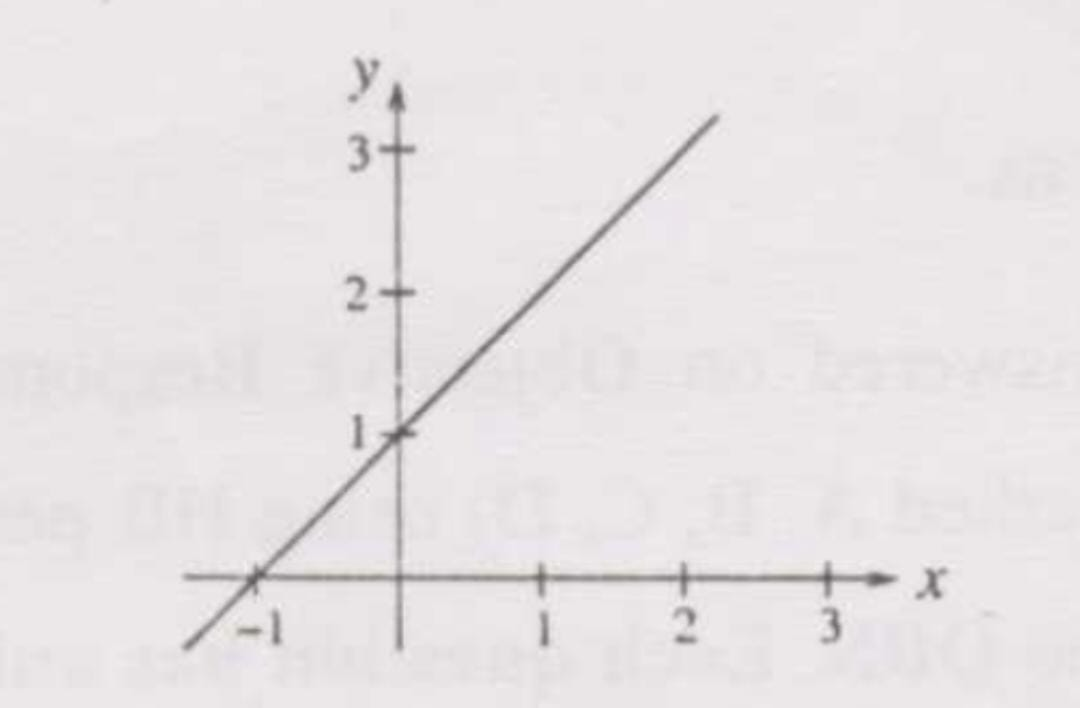
\includegraphics[width=0.4\textwidth]{figs/2007/EC/Q2.jpg}
    \caption{}
    \label{fig:Q2.jpg}
\end{figure}


\begin{enumerate}
\begin{multicols}{4}
    \item 1.0
    \item 2.5
    \item 4.0
    \item 5.0
\end{multicols} 
\end{enumerate}


\item For $|x| < 1 $, $ \coth(x)$ can be approximated as: 
\hfill{\brak{\text{EC 2007}}}
\begin{enumerate}
\begin{multicols}{4}
    \item $ x $
    \item $ x^2 $
    \item $ \frac{1}{x} $
    \item $ \frac{1}{x^2} $
\end{multicols} 
\end{enumerate}

\item $ \lim_{\theta \to 0} \frac{\sin(\theta/2)}{\theta} $ is: 
\hfill{\brak{\text{EC 2007}}}
\begin{enumerate}
\begin{multicols}{4}
    \item 0.5
    \item 1
    \item 2
    \item Not defined
\end{multicols} 
\end{enumerate}

\item Which of the following functions is strictly bounded? 
\hfill{\brak{\text{EC 2007}}}
\begin{multicols}{4}
\begin{enumerate}
    \item $ \sin x $
    \item $ e^x $
    \item $ \cos x $
    \item $ x^2 $
\end{enumerate}
\end{multicols}

\item For the function $ e^{-x} $, the linear approximation around $ x = 2 $ is:
\hfill{\brak{\text{EC 2007}}}
\begin{enumerate}
    \item $ (3 - x)^2 $
    \item $ 1 - x $
    \item $ [3 + 2\sqrt{2} - (1 + \sqrt{2})x]e^2 $
    \item $ e^{-2} $
\end{enumerate}

\item The equation $x^2 + x^4 - 4x - 4 = 0$ is to be solved using Newton-Raphson. If $x = 2$ is the initial approximation, then the next approximation using this method will be:
\hfill{\brak{\text{EC 2007}}}

\begin{multicols}{4}
\begin{enumerate}
    \item $\frac{2}{3}$
    \item $\frac{4}{3}$
    \item $1$
    \item $\frac{3}{2}$   
\end{enumerate}
\end{multicols}
\item
A 5-point sequence $x[n]$ is given as $x[-3]=1$, $x[-2]=1$, $x[-1]=0,
x[0]=5$, $x[1]=15$. Let $X\left(e^{j\omega}\right)$ denote the discrete-time Fourier
transform of $x[n]$. The value of
$
\int_{-\pi}^{\pi} X\left(e^{4j\omega3}\right)\, d\omega
$
\hfill{\brak{\text{EC 2007}}}
\begin{multicols}{4}
\begin{enumerate}
  \item 5
  \item $10\pi$
  \item $16\pi$
  \item $5 + j10\pi$
\end{enumerate}
\end{multicols}

\item The $z$-transform $X[z]$ of a sequence $x[n]$ is given by
$
X[z]=\frac{0.5}{1-2z^{-1}}.
$
It is given that the region of convergence of $X[z]$ includes the unit circle. The value of $x[0]$ is: 
\hfill{\brak{\text{EC 2007}}}
\begin{multicols}{4}
\begin{enumerate}
    \item $-0.5$
    \item $0$
    \item $0.25$
    \item $0.5$
\end{enumerate}
\end{multicols}

\end{enumerate}


\section{Optimization}
\begin{enumerate}[label=\thesubsection.\arabic*,ref=\thesubsection.\theenumi]
    \item The minimum value of 
	    $$J(x) = x^2 - 7x + 30$$ occurs at
	    \hfill (AE 2007)
    \begin{multicols}{4}
    \begin{enumerate}
        \item $x = 7/2$ 
        \item $x = 7/30$ 
        \item $x = 30/7$ 
        \item $x = 30$
    \end{enumerate}
    \end{multicols}
\item Consider the function $f(x) = x^2 - x -2$. The maximum value of $f(x)$ in the closed interval $[-4,4]$ is:
\hfill{\brak{\text{EC 2007}}}
\begin{multicols}{4}
\begin{enumerate}
    \item 18
    \item 10
    \item $-2.25$
    \item Indeterminate
\end{enumerate}
\end{multicols}
\end{enumerate}


\section{Probability}
\begin{enumerate}[label=\thesubsection.\arabic*,ref=\thesubsection.\theenumi]
\item  For station X, the maximum one day rainfall with 25 years return period is 100 mm.
The probability of a one day rainfall equal to or greater than 100 mm at station X occurring at least once in 15 successive years is
\hfill(AG 2007)
\begin{multicols}{4}
\begin{enumerate}
  \item 0.458
  \item 0.500
  \item 0.637
  \item 0.990
\end{enumerate}
\end{multicols}
\item If the standard deviation of the spot speed of vehicles in a highway is $8.8 kmph$ and the mean speed of the vehicles is $33 kmph$, the coefficient of variation in speed is
\hfill{\brak{\text{CE 2007}}}
\begin{multicols}{4}
\begin{enumerate}
\item 0.1517
\item 0.1867
\item 0.2666
\item 0.3646
\end{enumerate}
\end{multicols}
\item Suppose we uniformly and randomly select a permutation from the $20!$ permutations of $1,2,3,...,20.$ What is the probability that $2$ appears at an earlier position than any other even number  in selected permutation ?
\hfill {(CS 2007)}
\begin{enumerate}
    \begin{multicols}{4}
    \item $\frac{1}{2}$   

    \item $\frac{1}{10}$

    \item $\frac{9!}{20!}$
  
    \item None of these
    \end{multicols}
\end{enumerate}
    \item There are $n$ stations in a slotted LAN. Each station attempts to transmit with a probability $p$ in each time slot. What is the probability that {ONLY} one station transmits in a given time slot?  
\hfill {(CS 2007)}
    \begin{enumerate}
    \begin{multicols}{4}
        \item $np(1-p)^{n-1}$
        \item $(1-p)^{n-1}$
        \item $p(1-p)^{n-1}$
        \item $1 - (1-p)^{n-1}$
        \end{multicols}
    \end{enumerate}

\item If $ E $ denotes expectation, the variance of a random variable $ X $ is given by:
\hfill{\brak{\text{EC 2007}}}
    \begin{multicols}{2}
\begin{enumerate}
    \item $ E[X^2] - E^2[X] $
    \item $ E[X^2] + E^2[X] $
    \item $ E[X^2] $
    \item $ E^2[X] $
\end{enumerate}
\end{multicols}
\item If $ R(\tau) $ is autocorrelation of real, WSS random process, which is NOT true: 
\hfill{\brak{\text{EC 2007}}}
\begin{enumerate}
    \item $ R(\tau) = R(-\tau) $
    \item $ |R(t)| \leq R(0) $
    \item $ R(\tau) = -R(-\tau) $
    \item Mean square value is $ R(0) $
\end{enumerate}

\item If $ S(f) $ is power spectral density of a real WSS random process, which is ALWAYS true: 

\hfill{\brak{\text{EC 2007}}}
\begin{multicols}{4}
\begin{enumerate}
    \item $ S(0) \geq S(f) $
    \item $ S(f) \geq 0 $
    \item $ S(-f) = -S(f) $
    \item $ \int S(f) df = 0 $
\end{enumerate}
\end{multicols}
\item An examination consists of two papers, Paper I and Paper II. The probability of failing in Paper I is 0.3 and that in Paper II is 0.2. Given that a student has failed in Paper II, the probability of failing in Paper I is 0.6. The probability of a student failing in both the papers is: 
\hfill{\brak{\text{EC 2007}}}
\begin{multicols}{4}
\begin{enumerate}
    \item 0.5
    \item 0.18
    \item 0.12
    \item 0.06
\end{enumerate}
\end{multicols}
\item During transmission over a binary channel, bit errors occur independently with probability $p$. The probability of {at most one} bit in error in a block of $n$ bits is: 
\hfill{\brak{\text{EC 2007}}}
\begin{multicols}{2}
    

\begin{enumerate}
    \item $p^n$
    \item $1-p^n$
    \item $np(1-p)^{n-1} + (1-p)^n$
    \item $1-(1-p)^n$
\end{enumerate}
\end{multicols}

\item  Two 4-ary signal constellations are shown. It is given that $\phi_1$ and $\phi_2$ constitute an orthonormal basis and four symbols in each are equiprobable. Let $N_0/2$ denote the power spectral density of white Gaussian noise. 
\hfill{\brak{\text{EC 2007}}}

\begin{figure}[H]
    \centering
    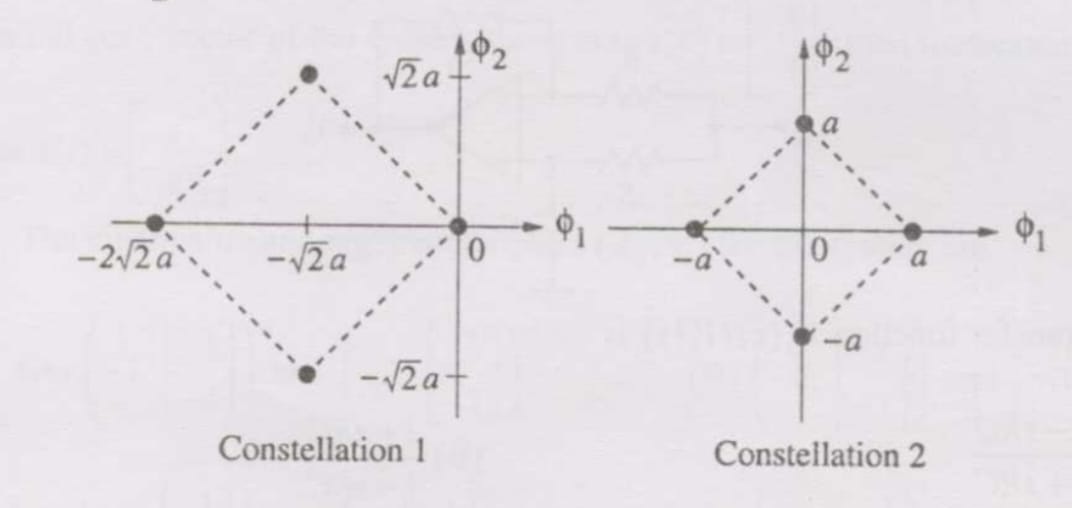
\includegraphics[width=0.6\textwidth]{figs/2007/EC/Q74Q75.jpg}
    \caption{}
    \label{fig:Q74@75.jpg}
\end{figure}

\begin{enumerate}
\item The ratio of the average energy of Constellation 1 to that of Constellation 2 is:
\begin{multicols}{4}
\begin{enumerate}
  \item $4a^2$
  \item $4$
  \item $2$
  \item $8$
\end{enumerate}
\end{multicols}


\item If these constellations are used over an AWGN channel, then:
\begin{enumerate}
  \item Probability of symbol error for Constellation 1 is lower
  \item Probability of symbol error for Constellation 1 is higher
  \item Probability of symbol error is equal for both
  \item Value of $N_0$ will determine which has lower error
\end{enumerate}
\end{enumerate}

\item
An input to a 6-level quantizer has PDF $f(x)$ as shown: it is piecewise-constant with three decision boundaries at $-1$, $0$, and $1$, chosen to maximize output entropy. The central plateau height is $a$, the outer flat region height is $b$. 
\hfill{\brak{\text{EC 2007}}}
\begin{figure}[H]
    \centering
    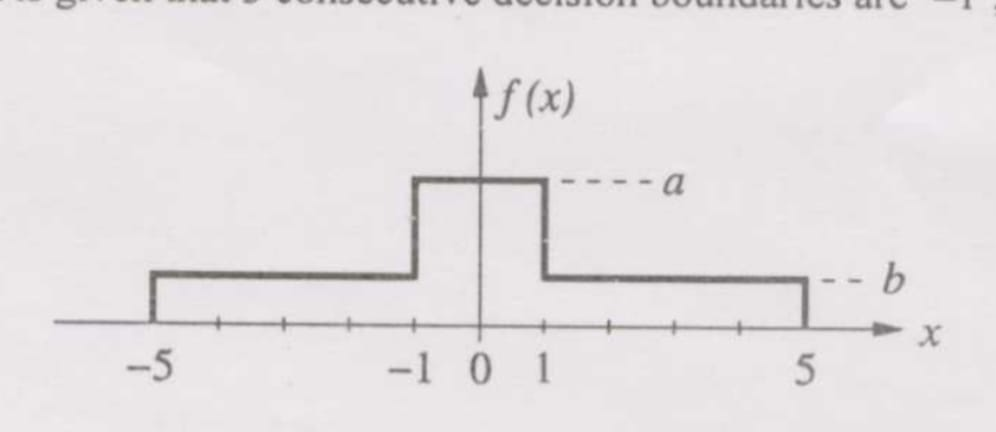
\includegraphics[width=0.4\textwidth]{figs/2007/EC/Q82Q83.jpg}
    \caption{}
    \label{fig:Q82Q83.jpg}
\end{figure}

\begin{enumerate}
\item The values of $a$ and $b$ are:
\begin{multicols}{4}
\begin{enumerate}
  \item $a=\tfrac{1}{6},\ b=\tfrac{1}{12}$
  \item $a=\tfrac{1}{5},\ b=\tfrac{3}{40}$
  \item $a=\tfrac{1}{4},\ b=\tfrac{1}{16}$
  \item $a=\tfrac{1}{3},\ b=\tfrac{1}{24}$
\end{enumerate}
\end{multicols}

\item Assuming reconstruction levels are midpoints of decision intervals, the ratio of signal power to quantization noise power is:

\begin{multicols}{4}
\begin{enumerate}
  \item $\frac{152}{9}$
  \item $\frac{64}{3}$
  \item $\frac{76}{3}$
  \item $28$
\end{enumerate}
\end{multicols}
\end{enumerate}

\item  A loaded dice has following probability distribution of occurrences
%
\begin{center}
\begin{tabular}{|c|c|c|c|c|c|c|}
\hline
Dice value      & 1   & 2   & 3   & 4   & 5   & 6   \\
\hline
Probability     & $1/4$ & $1/8$ & $1/8$ & $1/8$ & $1/8$ & $1/4$ \\
\hline
\end{tabular}
\end{center}
%
If three identical dice as the above are thrown, the probability of occurrence of values 1, 5 and 6 on the three dice is\hfill{(EE 2007)} 
% 
\begin{enumerate}
    \item same as that of occurrence of 3, 4, 5
    \item same as that of occurrence of 1, 2, 5
    \item$1/128$
    \item $5/8$
\end{enumerate}
%
\item A coin is tossed thrice. Let X be the event that head occurs in each of the first two tosses.  
Let Y be the event that a tail occurs on the third toss.  
Let Z be the event that two tails occur in three tosses.  
Based on the above information, which one of the following statements is TRUE?  
\hfill (GE 2007)
\begin{multicols}{2}
\begin{enumerate}
\item X and Y are not independent  
\item Y and Z are dependent  
\item Y and Z are independent  
\item X and Z are independent  
\end{enumerate}
\end{multicols}
\item Assume that the duration in minutes of a telephone conversation follows the exponential distribution $$f(x) = \frac{1}{5} e^{-x/5}, x \geq 0$$. The probability that the conversation will exceed five minutes is  
\hfill(IN 2007)
\begin{multicols}{4}
\begin{enumerate}
\item $\frac{1}{e}$  
\item $\frac{1}{5}$  
\item $\frac{1}{3}$  
\item $1 - \frac{1}{e}$  
\end{enumerate}
\end{multicols}
\item Two sensors have measurement errors that are Gaussian distributed with zero means and variances $\sigma_1^2$ and $\sigma_2^2$, respectively. The two sensor measurements $x_1$ and $x_2$ are combined to form the weighted average $x = \alpha x_1 + (1-\alpha)x_2, \, 0 \leq \alpha \leq 1$. Assuming that the measurement errors of the two sensors are uncorrelated, the weighting factor $\alpha$ that yields the smallest error variance of $x$ is  
\hfill(IN 2007)
\begin{multicols}{4}
\begin{enumerate}
\item $\frac{\sigma_1^2}{\sigma_1^2 + \sigma_2^2}$  
\item $\frac{\sigma_2^2}{\sigma_1^2 + \sigma_2^2}$  
\item $\frac{\sigma_1}{\sigma_1 + \sigma_2}$  
\item 0.5  
\end{enumerate}
\end{multicols}

\item The value of the integral $\int_{0}^{\infty} \int_{0}^{\infty} e^{-x^2-y^2} \, dx\, dy$ is  
\hfill(IN 2007)
\begin{multicols}{4}
\begin{enumerate}
\item $\sqrt{\pi}/2$  
\item $\sqrt{\pi}$  
\item $\pi$  
\item $\pi/4$  
\end{enumerate}
\end{multicols}

\end{enumerate}


\end{document}


